\chapter{Requirements and constraints}

\section{Functional Analysis}
The first step in determining the requirements for the aircraft is looking at its function in detail. This can be done using a functional flow diagram (FFD), which analyses a typical mission of the aircraft. From that, key functions can be identified and later formatted as a functional breakdown structure (FBS). The two diagrams are available as  A3 PDF pages at the end of this chapter.



\section{Requirement Discovery Tree}
In order to identify the system requirements based on the user requirements and project objectives, a requirement discovery tree has been generated (\autoref{fig:req_discovery_tree}). The tree starts with the requirement for designing a flying test bed for testing flexible wings, which is split into the requirement to perform the flight test and the requirement to satisfy the constraints. Since the functional requirements stem directly from the functions that the design has to be able to do, the Functional Breakdown is referenced.

The constraints are split into complying with budgets (mass, payload volume, electricity, internal volume, link, thrust, van volume, cost, payload aerodynamic, c.g.), airworthiness requirements, manufacturability, lifetime, sustainability, being unmanned, and withstanding ogf transonic loads.




\begin{figure}[h]
    \centering
    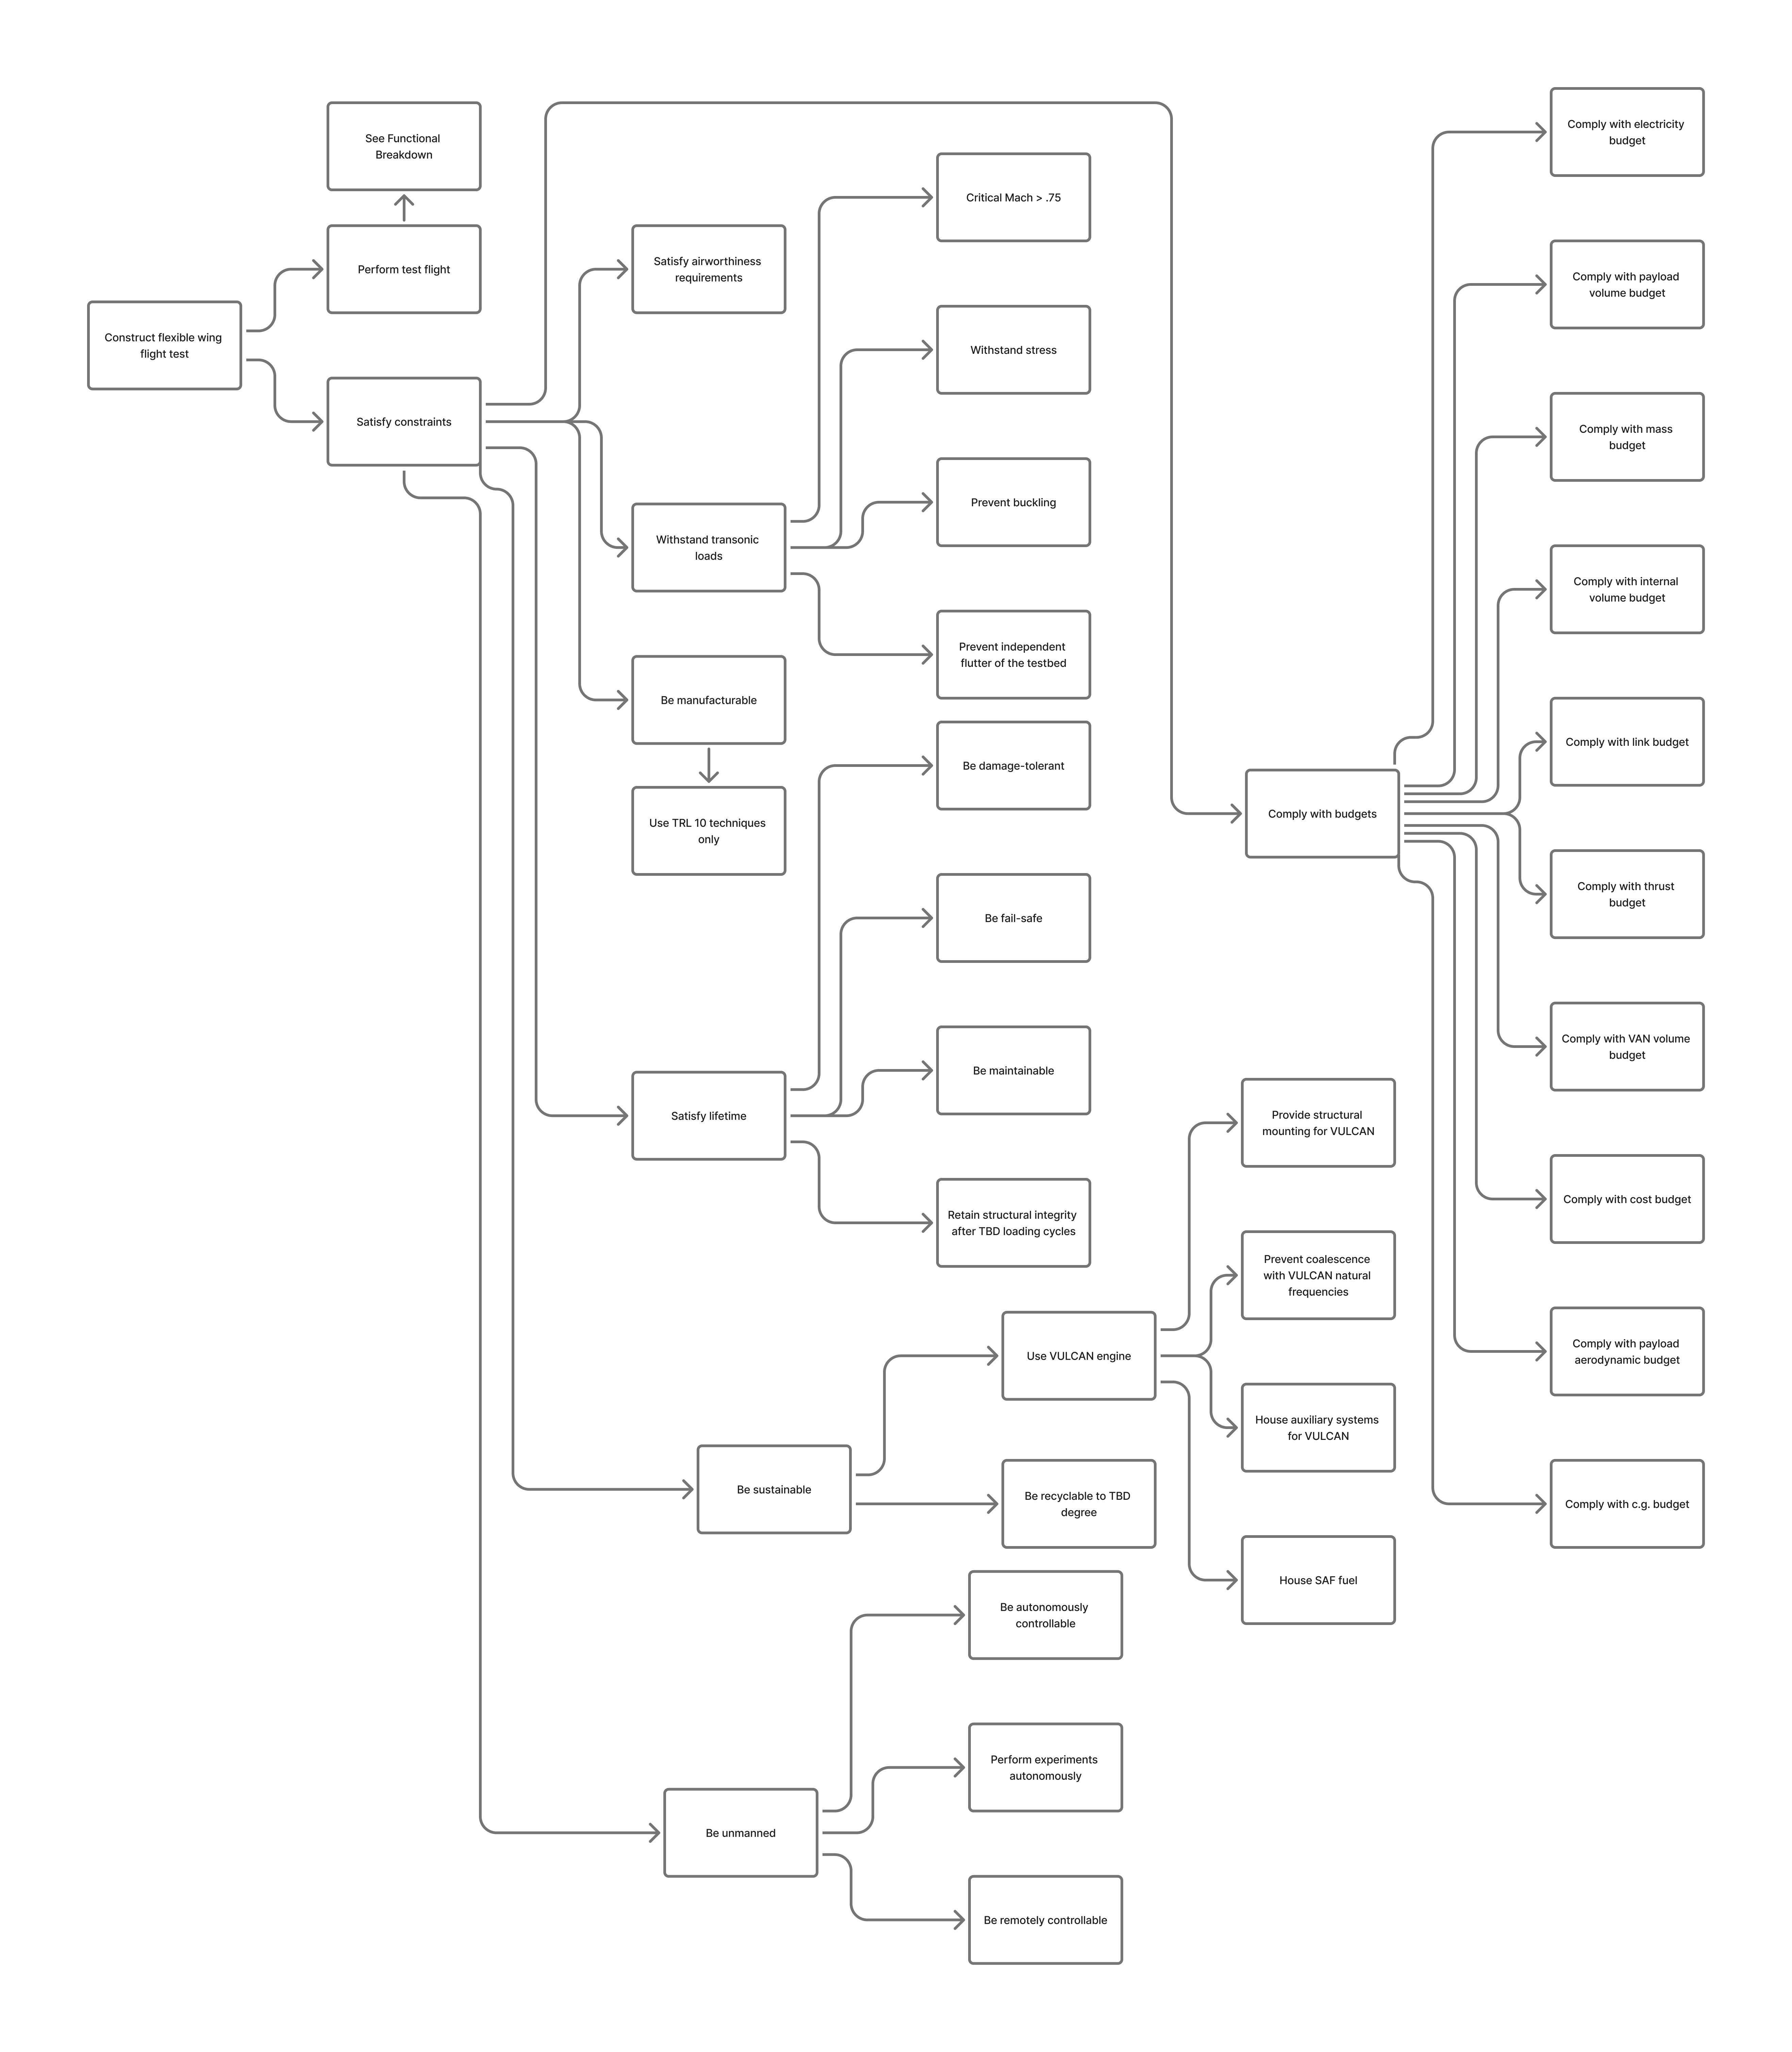
\includegraphics[width=1.0\linewidth]{figures/Flexible Wing Flight Requirements.png}
    \caption{Requirement Discovery Tree}
    \label{fig:req_discovery_tree}
\end{figure}

\section{Final list of system requirements}
The system requirements are divided into several categories: general (GEN), performance (PER), aerodynamics (AER), operations (OPS), certifications (CER), sustainability (SUS), control (CON), stability (STA), and structures (STR).

\begin{longtable}{|p{3cm}|p{11cm}|}
\caption{Top-level aircraft requirements}
\label{tab:system_requirements} \\
\hline
\textbf{Requirement ID} & \textbf{Requirement} \\
\hline
\endfirsthead

\hline
\textbf{Requirement ID} & \textbf{Requirement} \\
\hline
\endhead

& The aircraft shall allow for performing flight tests.\\ \hline 

& The aircraft shall satisfy airworthiness requirements.\\ \hline 

& The aircraft shall withstand transonic loads.\\ \hline

& The aircraft shall have a critical Mach number larger than 0.75, with a margin of TBD.\\ \hline

& The aircraft structure shall withstand stresses at Mach 0.75 with a margin of TBD. \\\hline

& The aircraft structure shall not buckle below Mach 0.75 \\\hline

& The flutter speed of the test bed shall be above Mach 0.75 to allow for transonic tests. \\\hline

& The aircraft shall be manufacturable \\ \hline

& It shall be possible to manufacture the aircraft using TRL 10 techniques. \\ \hline


& The lifetime of the aircraft shall be longer than 15 years. \\ \hline

& The aircraft shall be damage-tolerant. \\ \hline

& The aircraft shall be fail-safe. \\ \hline

& The aircraft shall be maintainable. \\ \hline

& The aircraft shall retain structural integrity after TBD loading cycles, including a margin of TBD. \\ \hline

& The aircraft shall comply with budgets. \\ \hline

& The aircraft shall comply with budgets. \\ \hline


GEN-001 & The total mass shall not be larger than 50 kg. \\ \hline
GEN-002 & The total cost of a single configuration shall not exceed 45k€. \\ \hline
GEN-003 & The available payload mass shall be larger than 5 kg. \\ \hline
GEN-004 & The VULCAN engine shall be used by all aircraft configurations. \\ \hline

PER-001 & The endurance at maximum payload shall be longer than 30 minutes. \\ \hline
PER-002 & The aircraft shall be able to sustain Mach 0.75 for TBD min. \\ \hline
PER-003 & The aircraft shall be able to sustain the speed faster than Mach 0.4 during the main flight stage. \\ \hline

AER-001 & The critical Mach number shall be higher than 0.75. \\ \hline

OPS-001 & The lifetime of a single configuration shall be longer than 15 years. \\ \hline
OPS-002 & All regular service, required parts, and tools shall fit within a van-sized vehicle of TBDexact dimensions. \\ \hline
OPS-003 & It shall be possible to maintain the aircraft on a regular basis. \\ \hline

CER-001 & The aircraft shall not exceed an altitude of TBD. \\ \hline
CER-002 & It shall be possible to safely recover the aircraft in all flight scenarios. \\ \hline

SUS-001 & The aircraft shall use sustainable aviation fuel (SAF). \\ \hline
SUS-002 & The aircraft shall be recyclable. \\ \hline

CON-001 & The aircraft shall be capable of autonomous flight. \\ \hline
CON-002 & The aircraft shall be fully controllable remotely. \\ \hline

STA-001 & The aircraft shall be capable of stable, neutral, and unstable flight conditions. \\ \hline

STR-001 & The structure shall withstand transonic loads. \\ \hline
STR-002 & The structure shall allow integration of the VULCAN engine. \\ \hline
STR-003 & The structure shall accommodate a payload bay of at least 5 litres. \\ \hline
STR-004 & The structure shall accommodate space for a secondary flight computer. \\ \hline
STR-005 & The wing, tail, and payload bay shall be modular. \\ \hline
STR-006 & The aircraft shall provide interfaces for mounting sensors and actuators. \\ \hline

\end{longtable}

\textcolor{red}{Drive and killer requirements, etc.}

\textcolor{red}{Deriving more detailed requirements}

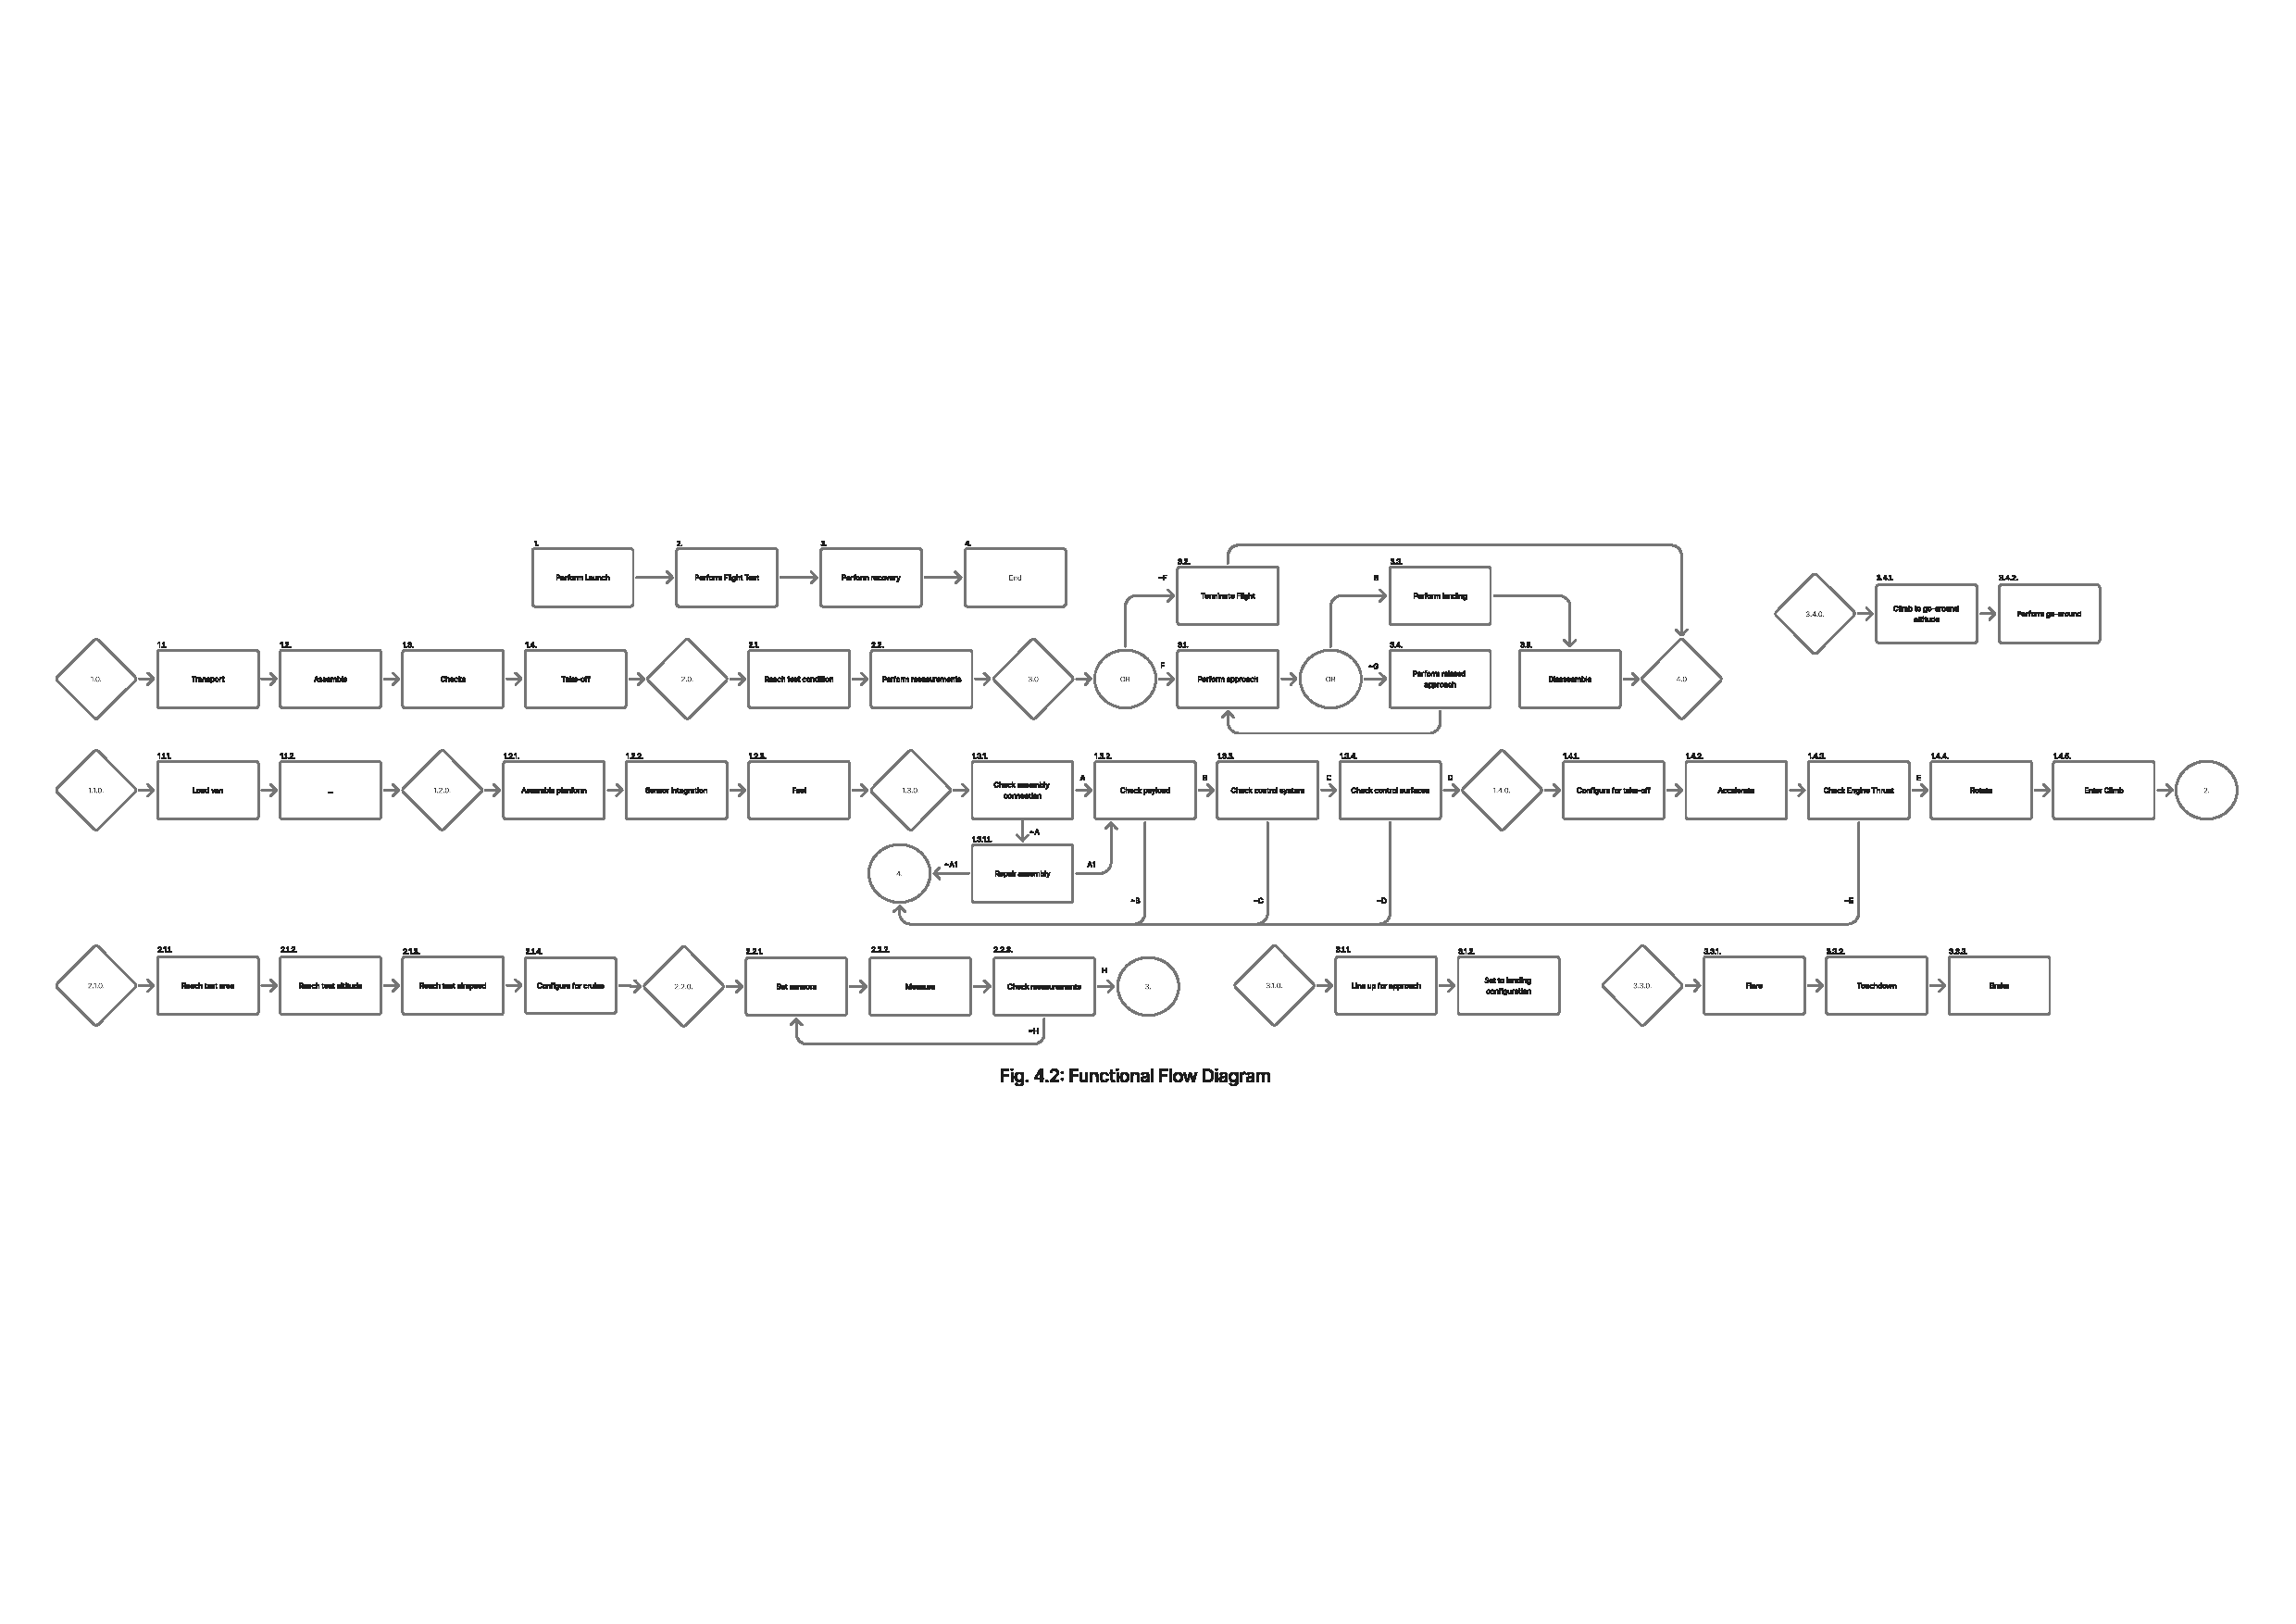
\includepdf[pages=-,fitpaper=true, width=420mm, keepaspectratio]{figures/Functional Flow Diagram.pdf}


\includepdf[pages=-,fitpaper=true, width=420mm, keepaspectratio]{figures/Functional Breakdown Structure.pdf}